\title{Microkernel Architecture}
\author{Richard Thomas}
\date{\week{3}}

\maketitle

\section{Introduction}

The microkernel architecture aims to deliver sophisticated software systems while maintaining the quality attributes of simplicity and extensibility.
This is achieved by implementing a simple core system that is extended by plug-ins that deliver additional system behaviour.
Microkernel is also known as a ``plug-in'' architecture.

Many common applications use the microkernel architecture.
Web browsers, many IDEs (notably Eclipse), Jenkins, and other tools all use this architecture.
They deliver their core functionality and provide a plug-in interface that allows it to be extended.
\link{Eclipse}{https://www.eclipse.org/downloads/packages/} is famous as a simple text editor that
can be extended to be a sophisticated software development tool through its plug-in interface.

\vspace{2mm}
\begin{definition}[Microkernel Architecture]
    A core system providing interfaces that allow plug-ins to extend its functionality.
\end{definition}

\begin{figure}[h!]
    \centering
    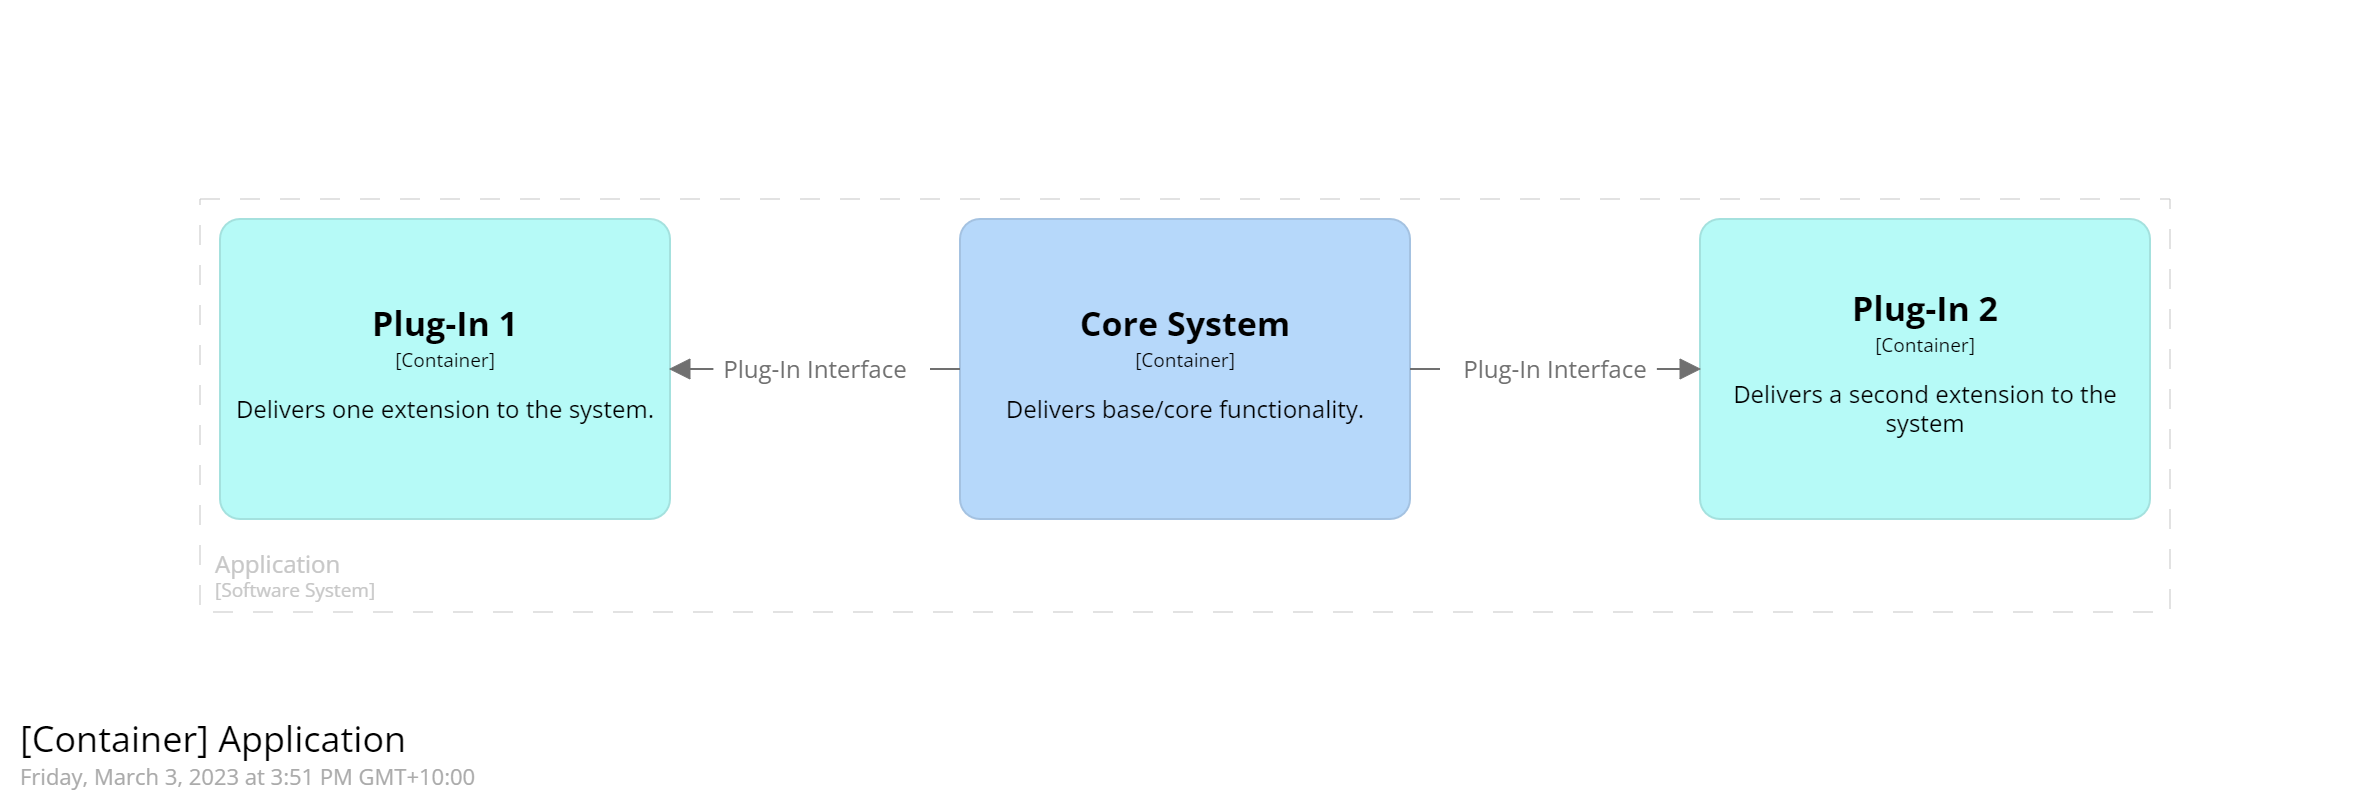
\includegraphics[trim=38 120 22 110,clip,width=0.85\textwidth]{diagrams/generic-microkernel.png}
    \caption{Microkernel architecture -- generic structure.}
    \label{fig:microkernel}
\end{figure}

For example, a web browser provides the core behaviour of rendering web pages.
Plug-ins extend the browser with specialised behaviour, such as a PDF viewer or dark mode reader.


\section{Terminology}

The microkernel architecture consists of four elements.
The \emph{core system}, \emph{plug-ins} and \emph{plug-in interface} shown in figure \ref{fig:microkernel}, plus a \emph{registry}.

\begin{description}
    \item[Core system] implements the system's base functionality.
    \item[Plug-ins] extend the system by providing independent, specialised behaviour.
    \item[Plug-in interface] describes how the core system and plug-ins interact.
    \item[Registry] tracks which plug-ins are available to the core system and how to access them.
\end{description}

The core system implements the minimal functionality that provides the base, or framework, of the system.
This may be the core functionality of the system, like the Eclipse text editor or a web browser's page rendering engine.
Alternatively, the core system may implement a general processing path, like a payroll system's payment process.

The payment process may be simply, identify an employee, calculate their fortnightly pay, and send payment to their bank account.
Calculating pay can be a very complex process\footnote{See the Queensland Health payroll disaster
\url{https://www.henricodolfing.com/2019/12/project-failure-case-study-queensland-health.html}}.
There are different pay rates, bonuses, incentives, salaried staff, staff paid commission, staff paid hourly rates,
overtime rates, penalty rates, deductions, taxes, and many other pay related calculations to consider for each individual.

Plug-ins are independent components that extend the behaviour of the core system.
The simple approach is that the system is delivered as a monolith, including the core system and the plug-in.
In this case the core system uses the plug-in via a method invocation.

In the payroll example, plug-ins can remove the complexity of different pay adjustment calculations from the core system, by moving each calculation to a separate component.
This also improves extensibility, maintainability and testability of the system.
New calculations can be added to the system by implementing a new plug-in.
As each plug-in is independent of the others, it is easier to implement a new calculation, or changing an existing one, than trying to do so in a large monolith.
New plug-ins can be tested independently and then integrated into the system for system testing.

There is usually a single standard interface between the core system and the plug-ins for a domain.
The interface defines the methods that the core system can invoke, data passed to the plug-in, and data returned from the plug-in.
The plug-in component implements the interface and delegates responsibilities within the component to deliver its behaviour.

Figure \ref{fig:interface} is an example of a possible interface for the pay adjusment calculation plug-ins.
Each pay adjustment plug-in returns a \texttt{MonetaryAmount} indicating the amount by which the employee's base pay is to be adjusted in the pay period.
The amount may be positive or negative.
The \texttt{employee}, \texttt{periodDetails}, \texttt{employeeConditions} and \texttt{basePay} objects are passed as parameters to the plug-in.
The plug-in can extract the data it needs from these objects to perform its calculation.
The \texttt{periodDetails} object provides data about the work performed by the employee during the pay period (e.g. time worked, overtime, higher duties adjustments, ...).
The \texttt{employeeConditions} set provides data about each of the employee's pay conditions (e.g. before tax deductions, union membership, ...).

\begin{figure}[ht]{\textwidth}
\centering
\begin{shaded}
\begin{lstlisting}[style=java]
public interface PayAdjustmentPlugin {
    public MonetaryAmount adjustPay(Employee employee,
                                    WorkDetail periodDetails,
                                    Set<Condition> employeeConditions,
                                    MonetaryAmount basePay);
}
\end{lstlisting}
\end{shaded}
\caption{Example plug-in interface for payroll system.}
\label{fig:interface}
\end{figure}

The registery records which plug-ins are available to the core system and how they are accessed.
For the simple case of plug-ins being used by method invocation,
the registry just needs to record the name of the plug-in and a reference to the object that implements the plug-in's interface.
For the payroll example, this could be a simple map data structure.
The core system could lookup a plug-in by its name and then apply it by invoking the \texttt{adjustPay} method on the plug-in object.

\section{Microkernel Principles}
While the concept of a microkernel architecture is straightforward,
there are some principles which should be maintained to produce a maintainable and extendable architecture.

\begin{definition}[Independent Plug-in Principle]
    Plug-ins should be independent, with no dependencies on other plug-ins.
    The only dependency on the core system is through the plug-in interface.
\end{definition}

Plug-ins should be independent of each other.
If a plug-in depends on other plug-ins it increases the complexity of the design.
This complexity is called \link{\emph{coupling}}{https://leanpub.com/isaqbglossary/read\#term-coupling},
which is a measure of how dependent different parts of a system are on each other \cite{glossary-architecture}.
High coupling (many dependencies) makes it difficult to understand the software,
which in turn makes it difficult to modify and test the software.
Consequently, if a plug-in depends on other plug-ins it requires understanding the dependencies on the other plug-ins to modify or test the plug-in
This can lead to an architecture that resembles a ``big ball of mud''.

Plug-ins and the core system should be \emph{loosely} coupled.
The core system should only depend on the plug-in interface and data returned via that interface, not any implementation details of individual plug-ins.
Plug-ins should only depend on the data passed to them via the plug-in interface.
Plug-ins should not rely on implementation details of the core system, nor its datastore.
If plug-ins and the core system are not isolated from each other by an interface,
then any changes to the core system may require changes to some or all of the plug-ins.
Similarly, the plug-in interface should mean that any changes to the plug-in will have no impact on the core system.

\begin{definition}[Standard Interface Principle]
    There should be a single interface that defines how the core system uses plug-ins.
\end{definition}

To provide an extensible design, the core system needs a standard way to use plug-ins.
This means that the plug-in interface needs to be the same for all plug-ins.
That way the core system can use any plug-in without needing to know details about how the plug-in is implemented.
This again is about reducing coupling between the core system and the plug-ins.
The standard interface principle means that there is no additional complexity if the core system uses two plug-ins or thousands of plug-ins.


\section{Architecture Partitioning}

\begin{wrapfigure}{r}{0.32\textwidth}
    \vspace{-20pt}
    \centering
    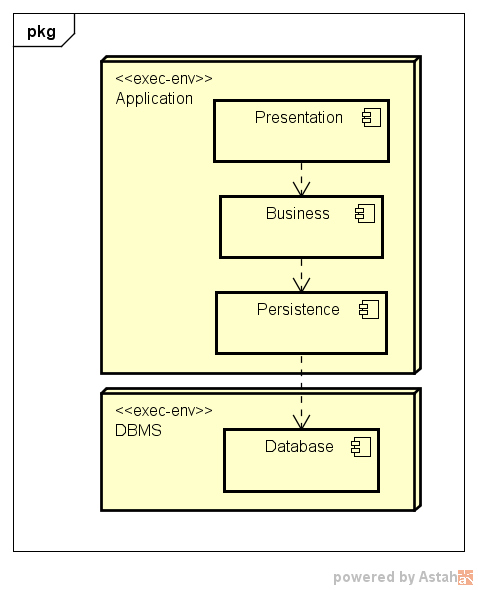
\includegraphics[trim=74 58 40 41,clip,width=0.3\textwidth]{diagrams/technical-partitioning.png}
    \caption{Layered architecture as example of technical partitioning.}
    \label{fig:technical-partitioning}
\end{wrapfigure}

\subsection{Technical Partitioning}
The notes about \link{layered architecture}{https://csse6400.uqcloud.net/handouts/layered.pdf}
described the idea of partitioning an architecture into layers, as in figure \ref{fig:technical-partitioning}.

This approach to partitioning the architecture is called \emph{technical partitioning}.
Each layer represents a different technical capability.
The presentation layer deals with user interaction.
The business layer deals with the application's core logic.
The persistence layer deals with storing and loading data.
The database layer deals with file storage and access details.

Technical partitioning corresponds to how developers view the code.
Its advantage is that all related code resides in a single layer of the architecture,
making each layer \link{cohesive}{https://leanpub.com/isaqbglossary/read\#term-cohesion} from a technical perspective.
This makes it easier to work with different parts of the code that deal with the same technical capability.
The \emph{layer isolation}, \emph{neighbour communication}, \emph{downward dependency},
and \emph{upward notification} principles help reduce coupling between layers.

\clearpage
\subsection{Domain Partitioning}
An alternative partitioning approach is called \emph{domain partitioning}.
In domain parititioning, the architecture is split into partitions (or major components)
corresponding to independent business processes or workflows (the \emph{domains}).
Figure \ref{fig:domain-partitioning} is an example of domain partitioning for an on-line store, similar to the
Sahara eCommerce example from the \link{architectural views}{https://csse6400.uqcloud.net/handouts/views.pdf} notes.

\begin{figure}[h!]
    \centering
    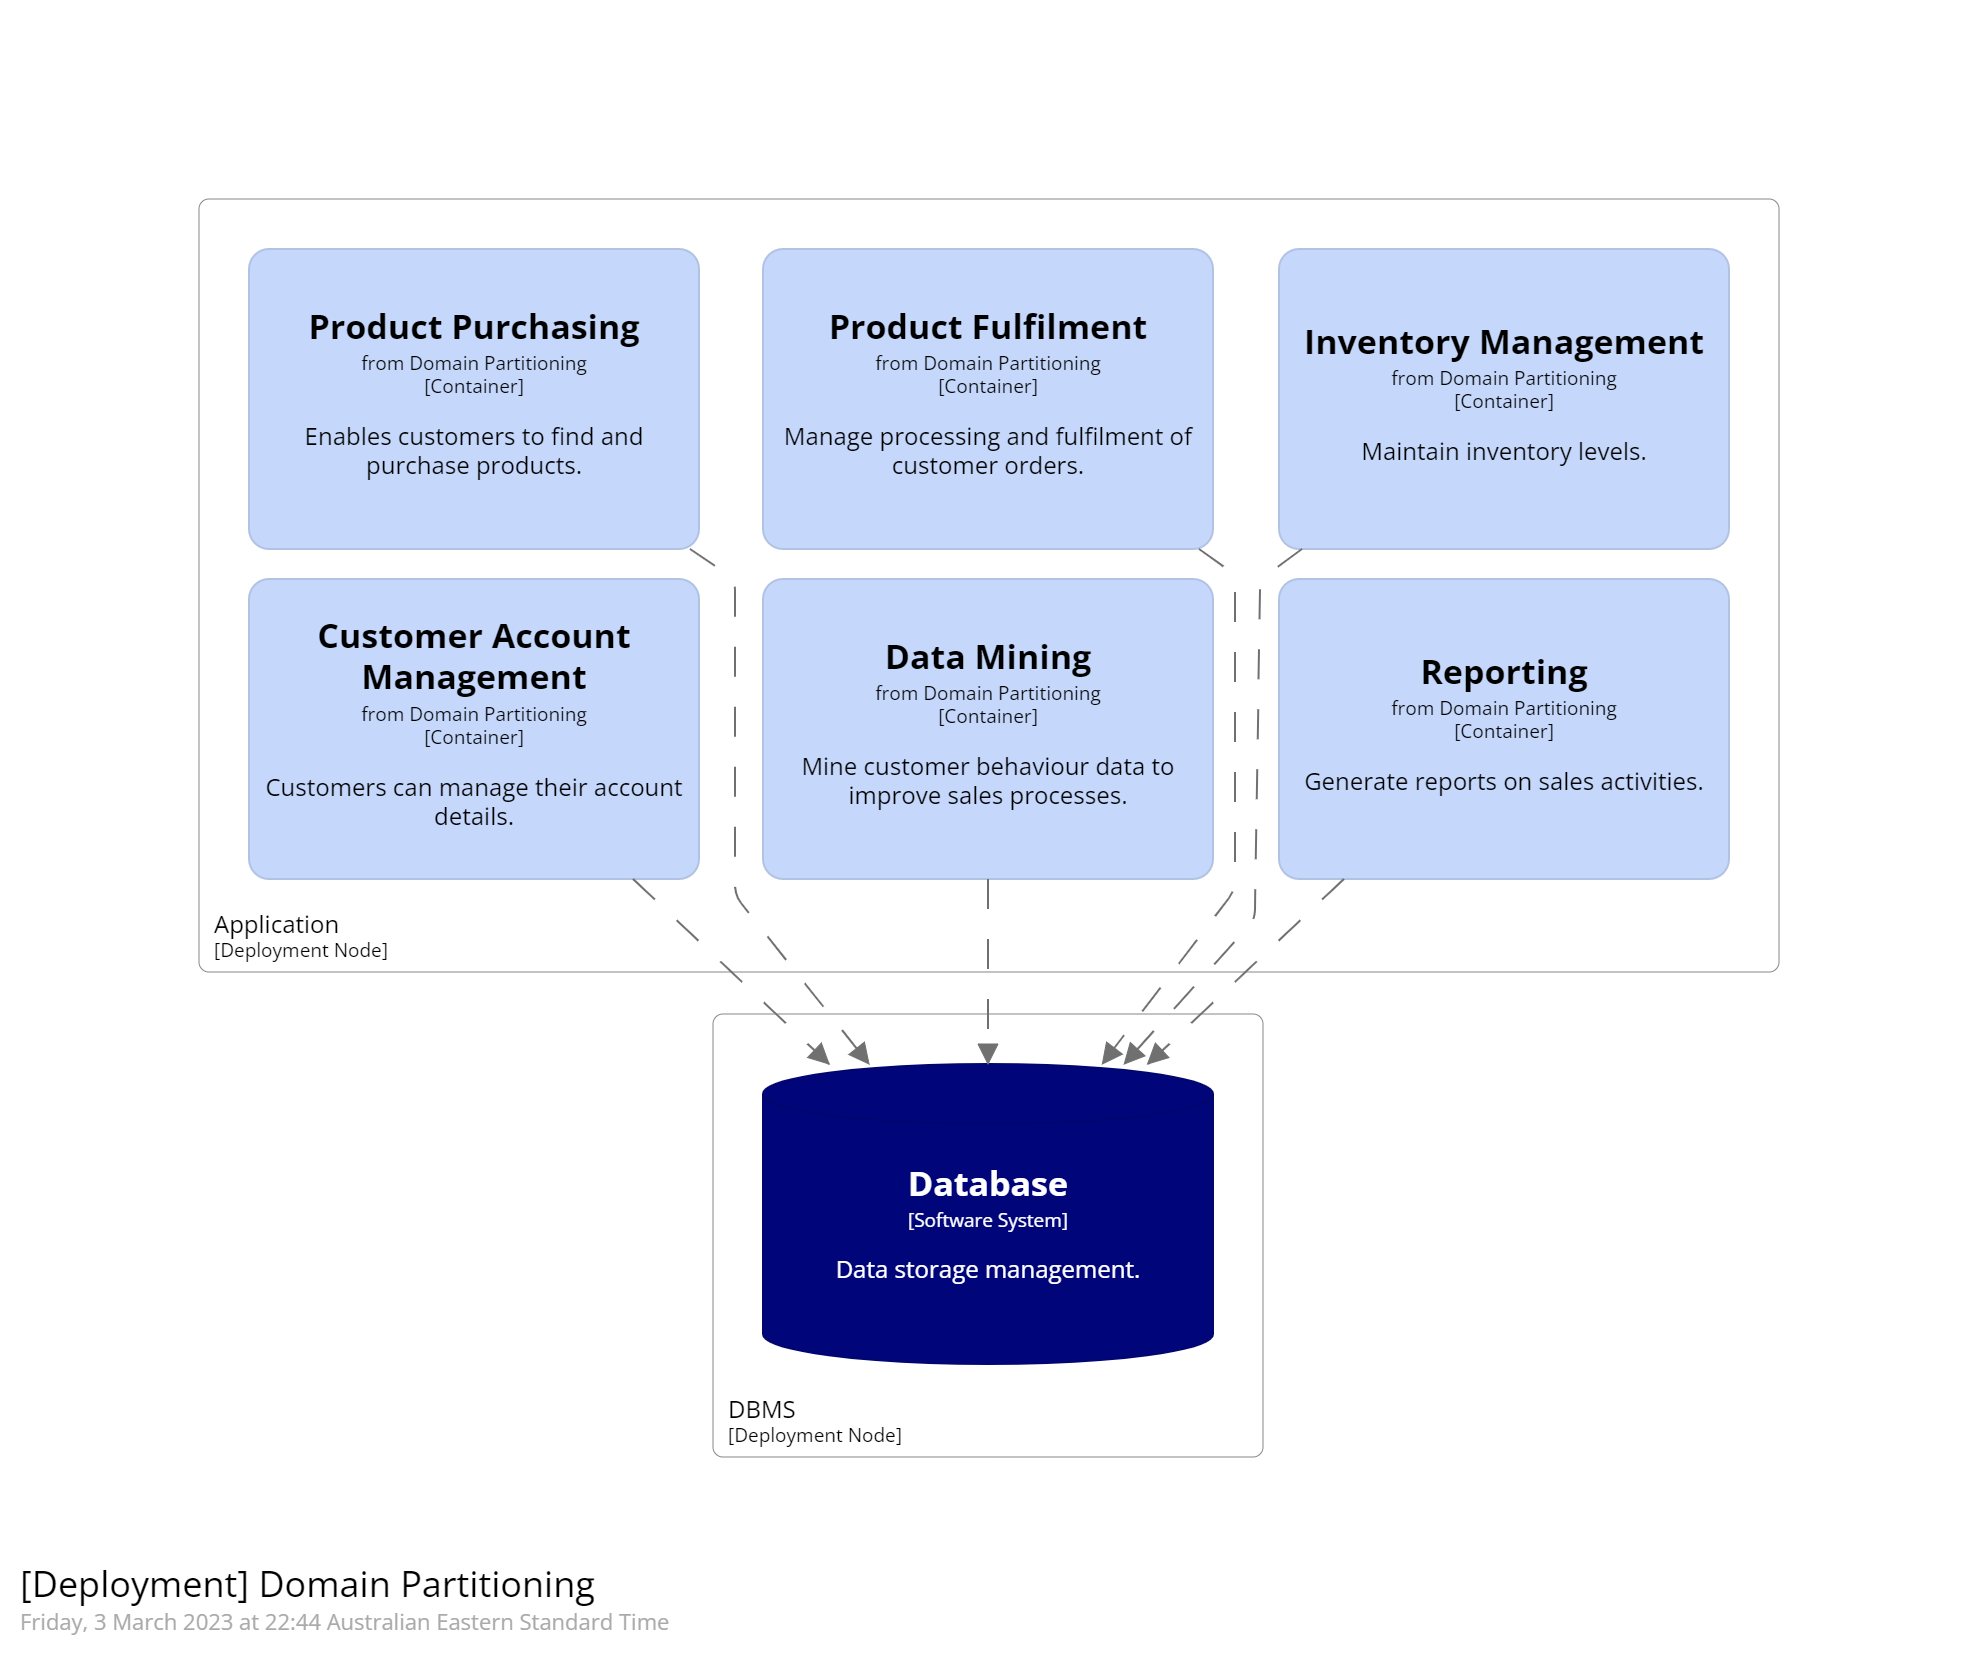
\includegraphics[trim=38 42 19 44,clip,width=0.9\textwidth]{diagrams/domain-partitioning.png}
    \caption{Example of domain partitioning.}
    \label{fig:domain-partitioning}
\end{figure}

In this approach, each domain is independent of the others.
The components within the domain partition are responsible for delivering all of that workflow's behaviour.
The advantage of this is that it fits well with an agile delivery focus.
A single user story will be implemented entirely within one domain.
This also makes it easier to implement multiple user stories concurrently, if they are all from different domains.
Eric Evans popularised domain partitioning in his book \textit{Domain-Driven Design} \cite{ddd-evans}.

\todo{More detail about advantages and disadvantages of technical vs domain partitioning.}


\section{Extensions}

While the core system is often a monolith and it, along with all its plug-ins, is often deployed as a single monolith
(e.g. a web browser), that is not the only approach to using the microkernel architecture.

\todo{Describe variations on the microkernel architecture and distribution options.
This includes using the Adapter design pattern for components that don't implement the standard interface.}


\section{Conclusion}

%A pipeline architecture is a good choice for data processing when interactivity is not a concern.
%Conceptually pipelines are very simple.
%Following the principles of a pipeline architecture will deliver a modular system which supports high reuse.
